% !TeX spellcheck = en_US 
\documentclass[proposal]{byu-aero}

\usepackage{lipsum}

%!!!!!!!!!!!!!!!!!!!!!!!!!!!!!!!!!!!!!!!!!!!!!!!!!!!!!!!!!!!!!!!!!!!!!!!!!!!!!!!!!!!!!!!!%
%!!!!!!! UNLESS YOU KNOW WHAT YOU'RE DOING, DO NOT TOUCH ANYTHING ABOVE THIS LINE !!!!!!!%
%!!!!!!!!!!!!!!!!!!!!!!!!!!!!!!!!!!!!!!!!!!!!!!!!!!!!!!!!!!!!!!!!!!!!!!!!!!!!!!!!!!!!!!!!%

%%%%%%%%%%%%%%%%%%%%%%%%%%%%%%%%%%
%%%%%%%%%%   Text Body   %%%%%%%%%
%%%%%%%%%%%%%%%%%%%%%%%%%%%%%%%%%%
\begin{document}

%%%%%%%%%%%%%%%%%%%%%%%%%%%%%%%%%%%%%%%%%%%%%%%%%%%%%%%%%%%%%%%%%%%%%%%%%%%%%%%%%%%%%%%%%
%%%%%%%%%%%%%%%%%%%%%%%%%%%%         EXECUTIVE SUMMARY         %%%%%%%%%%%%%%%%%%%%%%%%%%
%%%%%%%%%%%%%%%%%%%%%%%%%%%%%%%%%%%%%%%%%%%%%%%%%%%%%%%%%%%%%%%%%%%%%%%%%%%%%%%%%%%%%%%%%

\section{Executive Summary} % (10 Points)
\label{sec:ExecutiveSummary}
% Section Requirements:
% 1) Objective Statement
% 2) Planned approach to achieve all objectives
% 3) \textbf{Includes main points from subsequent sections} (we lost points on this in 2020)

{\color{BYUred}[THIS WILL DEPEND ON THE SPECIFIC DETAILS FOR THIS YEAR'S COMPETITION.]}

{\color{BYUred}[STRONG OBJECTIVE STATEMENT.]}

{\color{BYUred}[SEVERAL SENTENCES ABOUT YOUR PLANNED APPROACH TO ACHIEVE ALL OBJECTIVES.]}
\lipsum[2]

{\color{BYUred}[PARAGRAPH COVERING MAIN POINTS FROM ALL THE SECTIONS IN THE PROPOSAL.]}
\lipsum[2]




%%%%%%%%%%%%%%%%%%%%%%%%%%%%%%%%%%%%%%%%%%%%%%%%%%%%%%%%%%%%%%%%%%%%%%%%%%%%%%%%%%%%%%%%%
%%%%%%%%%%%%%%%%%%%%%%%%%%%%         MANAGEMENT SUMMARY        %%%%%%%%%%%%%%%%%%%%%%%%%%
%%%%%%%%%%%%%%%%%%%%%%%%%%%%%%%%%%%%%%%%%%%%%%%%%%%%%%%%%%%%%%%%%%%%%%%%%%%%%%%%%%%%%%%%%

\section{Management Summary} % (40 Points)
\label{sec:ManagementSummary}
% Section Requirements:
% 1) Describe the organization, the roles of each team and individual skill sets required
% 2) Organization chart (by team/function, individual names are not required for the proposal)
% 4) Schedule / Major Milestone chart
% 5) Budget (not only for expected materials and manufacturing of the airplane, but for travel to the competition site and any other expenses associated with the competition)



%%%%%%%%%%%%%%%%%%%%%%%%%%%%%
%%% - Team Organization - %%%
%%%%%%%%%%%%%%%%%%%%%%%%%%%%%
\subsection{Team Organization}
\label{ssec:TeamOrganization}

%Team Organization Chart:
%TEAM ORGANIZATION
\begin{wrapfigure}[7]{R}{0in}
	\centering
	\raisebox{0pt}[\dimexpr\height-3\baselineskip\relax]{
\begin{tikzpicture}[node distance = 1cm, auto]

	% Place nodes
	\node [block] (Project Manager) {\footnotesize Project Manager};
%	\node [block, below left = 0.1 and -1.25cm  of Project Manager] (Engineering Lead) {\footnotesize Engineering Lead};
%	\node [block, below right = 0.1 and -1.25cm   of Project Manager] (Project Manager) {\footnotesize Project Manager};

	\node [block2, below left = 0.25 and -1.25cm of Project Manager] (Aerodynamics) {\footnotesize Aerodynamics};
	\node [block2, below left = 1.0 and -1.25cm  of Project Manager] (Structures) {\footnotesize Structures};
	\node [block2, below left = 1.75 and -1.25cm  of Project Manager] (Propulsion) {\footnotesize Propulsion};
	\node [block2, below right = 0.25 and -1.25cm  of Project Manager] (Systems) {\footnotesize Systems};
	\node [block2, below right = 1.0 and -1.25cm  of Project Manager] (Graphics) {\footnotesize Graphics};
	\node [block2, below right = 1.75 and -1.25cm  of Project Manager] (Manufacturing) {\footnotesize Manufacturing};

	% Draw edges
%	\path[line] let \p1=(Project Manager.south), \p2=(Engineering Lead.east) in (Project Manager.south) --  +(0,0.55*\y2) -| node {} (Engineering Lead.east);
%	\path[line] let \p1=(Project Manager.south), \p2=(Project Manager.west) in (Project Manager.south) -- +(0,0.55*\y2) -| node {} (Project Manager.west);

	\path[line] let \p1=(Project Manager.south), \p2=(Aerodynamics.east) in (Project Manager.south) -- +(0,0.65*\y2) -| node  {} (Aerodynamics.east);
	\path[line] let \p1=(Project Manager.south), \p2=(Systems.west) in (Project Manager.south) -- +(0,0.65*\y2) -| node  {} (Systems.west);

	\path[line] let \p1=(Project Manager.south), \p2=(Structures.east) in (Project Manager.south) -- +(0,0.8*\y2) -| node  {} (Structures.east);
	\path[line] let \p1=(Project Manager.south), \p2=(Graphics.west) in (Project Manager.south) -- +(0,0.8*\y2) -| node  {} (Graphics.west);

	\path[line] let \p1=(Project Manager.south), \p2=(Propulsion.east) in (Project Manager.south) -- +(0,0.85*\y2) -| node  {} (Propulsion.east);
	\path[line] let \p1=(Project Manager.south), \p2=(Manufacturing.west) in (Project Manager.south) -- +(0,0.85*\y2) -| node  {} (Manufacturing.west);
\end{tikzpicture}}
	\caption{Here we show the structure of, and assignment areas within, our team organization.}
	\label{fig:personnelassignments}
\end{wrapfigure} %You can change the team_organization.tex file to update this and it will automatically update in this file.


%Introduction
\Cref{fig:personnelassignments} depicts the overall organization of our team structure.  Each of the teams is lead by an individual who answers to the Engineering Lead and Project Manager.  The skills required for each position/team are as follows.




%Team role descriptions continued.
\subsubsection{Engineering Lead} As with the team leads, the Engineering Lead primarily requires good decision making and leadership skills, qualities the BYU Aero Club seeks to develop in all of its members.  In addition the Engineering Lead has a well rounded understanding of the various systems and both design and testing expertise.
%schedule/milestone chart (since it fits here better.)  Note that you must modify this in the ganttchart.tex file, compile that file, and then compile this file again if you change the schedule.
\begin{wrapfigure}[14]{R}{0pt}
	\centering
	\raisebox{0pt}[\dimexpr\height-.5\baselineskip\relax]{
	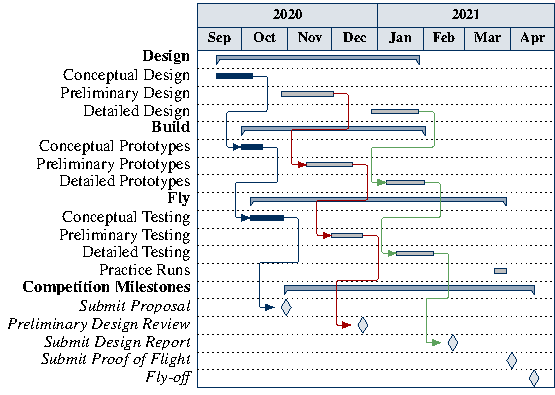
\includegraphics[width=0.45\textwidth]{ganttchart.pdf}}
	\caption{Our {\color{\BYUblue} Conceptual}, {\color{\BYUred} Preliminary}, and {\color{\BYUgreen} Detailed} design phases all culminate in internal design reviews, in addition to the required submissions.}
	\label{fig:plannedtiming}
\end{wrapfigure}
\subsubsection{Project Manager} The Project Manager has excellent organizational skills  and oversees the logistical side of the project: heading up report writing, budgeting tasks, scheduling, etc.
\subsubsection{Aerodynamics} The Aerodyanmics team members have expertise in aerodynamic analysis and testing, including skills in hand calculations, computational analysis tools, wind tunnel and glide testing.
\subsubsection{Structures} The Structures team members focus on skills in structural analysis and testing, employing hand calculations, computational tools, and various structural testing methods.
\subsubsection{Propulsion} The Propulsion team focuses on analyzing and testing the propulsion system effectiveness and efficiency, but also has skills in electronics related to the propulsion system.
\subsubsection{Systems} The Systems team works very closely with the Engineering Lead, as they oversee all systems interfacing, avionics, etc.  There is a sub-group of the Systems team that is assigned to work on the mission specific payload and related components, as well as related testing. %TODO: consider updating this sentence to reflect the actual specialized mission requirements for the year.
\subsubsection{Manufacturing} The Manufacturing team oversees the manufacturing of all prototypes and testing apparatus.
\subsubsection{Graphics} The Graphics team has skills in CAD design as well as graphical marketing for the team. 




%%%%%%%%%%%%%%%%%%%%%%%%%%%%%
%%%%%%%% - Timeline - %%%%%%%
%%%%%%%%%%%%%%%%%%%%%%%%%%%%%
\subsection{Schedule}
\label{ssec:Schedule}

%timeline description.
\Cref{fig:plannedtiming} depicts our planned timeline for the year. \Cref{sec:ManufacturingPlan,sec:TestingPlan} describe the flow of our schedule in more detail. Note that at the time of submitting this proposal, we have completed the conceptual design presented herein and have moved on to our preliminary design phase. Also of note is that we began prototyping early in order to apply a ``fail fast, fail often'' methodology to quickly fill any gaps in understanding and allow our underclassmen to develop their aircraft design intuition faster than if we waited to prototype after completing all the design phases.

%timeline figure included above since it looks better there.


%%%%%%%%%%%%%%%%%%
%%% - Budget - %%%
%%%%%%%%%%%%%%%%%%
\subsection{Budget}
\label{ssec:Budget}

%budget introduction
\Cref{tab:budget} contains a breakdown of our budget estimates for the \the\year-\NextYear competition year. Note that we have not allocated any funds to aircraft shipping costs as it is more cost effective for us to drive rather than fly to the fly-off location; therefore, we can transport our aircraft ourselves at no additional cost. %We lost points in 2020 for not explicitly saying this...

%Funding acquisition details
To obtain funding for our team this year, we will be {\color{BYUred}[NEED TO TALK ABOUT HOW YOU'RE GETTING FUNDS: CLUB, PREVIOUS YEARS WINNINGS, WEIDMANN CENTER, ETC.]} %we lost points in 2020 for not discussing this.
\lipsum[2]

% Project Budget
%TODO:	NEED TO FILL OUT THE DETAILS OF THIS BUDGET, HOW MANY OF EACH THINGS WILL YOU NEED? WILL YOU NEED OTHER THINGS? WILL YOU NOT NEED SOME THINGS LISTED HERE?
\begin{table}[htb!]
	\centering
	\renewcommand{\arraystretch}{1.2}
	\caption{Our project budget is broken down into several categories as well as individual items as shown here.}
	\label{tab:budget}
	\rowcolors{2}{BYUbluelite}{white}
	\begin{tabular}{ |l|l|l| } 
		\hline
		\rowcolor{BYUbluemid}
		Category & Items & Cost (\$) \\ 
		\hline
		Propulsion &  Brushless Motors (Qty?) | Propellers (Qty?) | ESCs (Qty?) &  \\
		\hline
		Power & (how many cells?) Lipo Batteries (Qty?) & \\ 
		\hline
		Structures & Balsa Wood (Qty?) | Monokote (Qty?) | ABS Filament (Qty?) | Foam (Qty?) & \\ 
		\hline
		Composites & Carbon Fiber Spars (Qty?) | Fiber Glass (Qty?) | Epoxy (Qty?) &  \\ 
		\hline
		Electronics & Servos (Qty?) | Receiver (Qty?) &  \\
		\hline
		Travel & Vehicle Rental | Gas (Qty?) &  \\
		\hline
		Food \& Lodging & Airbnb (Qty?) | Meals (Qty?) &  \\
		\hline 
		\textbf{Total Cost} & & \textbf{} \\ 
		\hline
		
	\end{tabular}
\end{table}






%%%%%%%%%%%%%%%%%%%%%%%%%%%%%%%%%%%%%%%%%%%%%%%%%%%%%%%%%%%%%%%%%%%%%%%%%%%%%%%%%%%%%%%%%
%%%%%%%%%%%%%%%%%%%%%%%%%%%%         CONCEPTUAL DESIGN         %%%%%%%%%%%%%%%%%%%%%%%%%%
%%%%%%%%%%%%%%%%%%%%%%%%%%%%%%%%%%%%%%%%%%%%%%%%%%%%%%%%%%%%%%%%%%%%%%%%%%%%%%%%%%%%%%%%%

\section{Conceptual Design Approach} % (20 Points)
\label{sec:ConceptualDesign}
% Section Requirements:
% 1) Decomposition of mission requirements into sub-system requirements.
% 2) Preliminary design / sizing results; concept sketch, if available (does not have to be representative of the final design) 
% 3) Sensitivity Study of Design Parameters



%%%%%%%%%%%%%%%%%%%%%%%%%%%%%
%%%% - Sub-system Reqs - %%%%
%%%%%%%%%%%%%%%%%%%%%%%%%%%%%
\subsection{Mission Requirements Decomposition}
\label{ssec:MissionReqs}

We have organized our sub-system requirements into aerodynamics, structure, propulsion, and specialty requirements explained below.

\subsubsection{Aerodynamics Requirements}
\label{sssec:AerodynamicReqs}

Some of the major requirements for the aerodynamics sub-system are: Maximize aerodynamic efficiency in order to use less energy to overcome drag for all flight missions.  Design wing loading to be able to take off and fly with design max payload weight.  Keep the wingspan within the maximum of {\color{BYUred}[MAX SPAN CONSTRAINT THIS YEAR]}.  Choose airfoil(s) and configuration that will make take off feasible in the {\color{BYUred}[THIS YEAR'S TAKE-OFF REQUIREMENT]}

\subsubsection{Structural Requirements}
\label{sssec:StructuralReqs}

The breakdown of mission requirements for the structures sub-system include: Minimize the structural weight while maintaining sufficient rigidity to keep the aerodynamics as designed, especially when full payload weight is in use.  Make sure the structure is sufficiently rigid to avoid aerodynamic flutter within the flight envelope. {\color{BYUred}[OTHER MISC. STRUCTURES REQUIREMENTS THIS YEAR (E.G. FOLDING WINGS.)]}

\subsubsection{Propulsion Requirements}
\label{sssec:PropulsionReqs}

The propulsion sub-system requirements are to: Have sufficient system efficiency and battery capacity to enable completion of the flight missions and maximizing speed with sufficient endurance while also providing sufficient thrust for {\color{BYUred}[THIS YEAR'S TAKE-OFF REQUIREMENT]}

\subsubsection{Specialty Requirements} %change this to be specifically what it is (like bomb drop or whatever the specific mission is)
\label{sssec:SpecialReqs}

{\color{BYUred}[REQUIREMENTS FOR THIS YEAR'S SPECIAL STUFF.]} 
\lipsum[2]



%%%%%%%%%%%%%%%%%%%%%%%%%%%%%%%%%%%%%
%%% - Preliminary Design/Sizing - %%%
%%%%%%%%%%%%%%%%%%%%%%%%%%%%%%%%%%%%%
\subsection{Preliminary Design}
\label{ssec:PreliminaryDesign}

%%%%%%%%%%%%%%%%%%%%%%%%%%%%%
%%%% - Concept Sketch - %%%%
%%%%%%%%%%%%%%%%%%%%%%%%%%%%%
%3 drawing views and rendered view of latest CAD models:  Make sure the aspect ratios match the draft figure names.
\begin{figure}[h!]
	\centering
	\begin{subfigure}[b]{0.475\textwidth}
		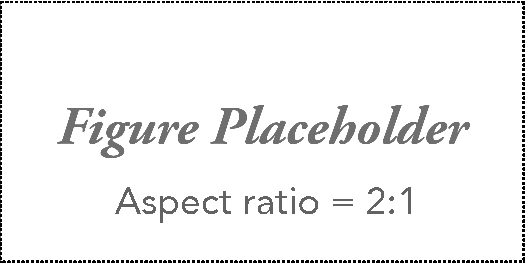
\includegraphics[width=\textwidth]{draft2x1}
		\caption{Top View}
		\label{fig:topview}
	\end{subfigure}
	%
	\begin{subfigure}[b]{0.475\textwidth}
		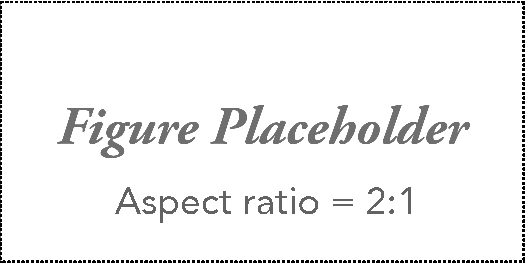
\includegraphics[width=\textwidth]{draft2x1}
		\caption{Side View}
		\label{fig:sideview}
	\end{subfigure}

	\begin{subfigure}[b]{0.475\textwidth}
		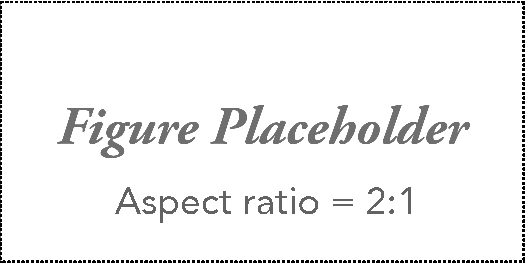
\includegraphics[width=\textwidth]{draft2x1}
		\caption{Front View}
		\label{fig:frontview}
	\end{subfigure}
	%
	\begin{subfigure}[b]{0.475\textwidth}
		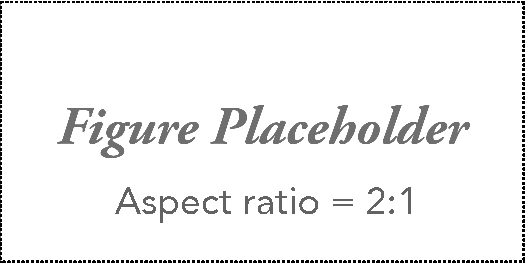
\includegraphics[width=\textwidth]{draft2x1}
		\caption{Rendered View}
		\label{fig:renderedview}
	\end{subfigure}
	\caption{Current drawings and rendering of our conceptual aircraft design.}
	\label{fig:prelimdrawings}
\end{figure}

%Preliminary design / sizing results

After making some decisions about the overall configuration of our aircraft (details on our decision process will be included in the Design Report), we arrived at the configuration seen in \cref{fig:prelimdrawings}.
{\color{BYUred}[COMMENT ON MAJOR FEATURES OF THE CONFIGURATION, GIVE SOME BASIC JUSTIFICATION, LIKE "WE CHOSE THIS BECAUSE IT WOULD WORK WELL FOR THIS REQUIREMENT"]}

Using common hand calculation level formulas, we arrived at a conceptual design with the following specifications: a wing span of {\color{BYUred} [X.X ft]}, aspect ratio of {\color{BYUred} [X.X]}, wing loading of {\color{BYUred} [X.X lbs/ft$^2$]}, horizontal and vertical tail volume ratios of {\color{BYUred} [X.X]} and {\color{BYUred} [X.X]} respectively, stall velocity of {\color{BYUred} [X.X ft/sec]}, and take-off distance of {\color{BYUred} [X.X ft]}.  {\color{BYUred}[INCLUDE ANY OTHER PERTINENT PARAMETERS HERE AS WELL!]}
{\color{BYUred}[DISCUSS ANY INTERESTING FEATURES SPECIFIC TO THIS YEAR'S REQUIREMENTS: ATTACHMENTS, FOLDING THINGS, DEPLOYMENT STUFF, ETC. THAT HAVE BEEN DECIDED IN THE CONCEPTUAL DESIGN.]}
\lipsum[1]



%%%%%%%%%%%%%%%%%%%%%%%%%%%%%%%
%%%% - Sensitivity Study - %%%%
%%%%%%%%%%%%%%%%%%%%%%%%%%%%%%%
\subsection{Sensitivity Study}
\label{ssec:SensitivityStudy}
%Sensitivity Study of Design Parameters.  This isn't just some linear plots of the ways to obtain points.  It's a sensitivity study of how the \textit{DESIGN PARAMETERS} relate to obtaining points. For example, how does weight affect the endurance and therefore number of laps that can be flown?
%In the code directory in the repository you found this template there is a sensitivity.jl code that produces the plot used here.

%Figure related to sensitivity study, move around to get formatting correct...
\begin{wrapfigure}[11]{R}{0pt}
	\centering
		\raisebox{0pt}[\dimexpr\height-2\baselineskip\relax]{
	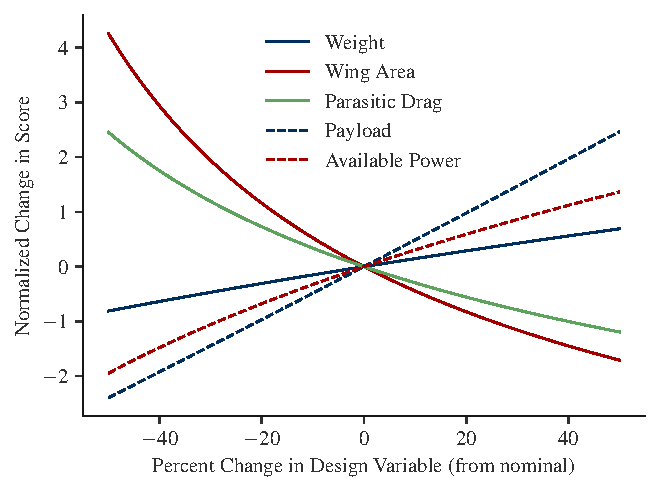
\includegraphics[width=3in]{sensitivityobj}
		}
	\caption{This plot shows the effects of those design parameters that directly affect the increase/decrease in mission scoring beyond simple completion.}
	\label{fig:sensitivity}
\end{wrapfigure}

For our sensitivity study, we first differentiated between design variables that could increase/decrease our score and those that were only related to the minimum constraints. Based on the scoring metrics, we found the parameters that could affect the score to be: wing area, aircraft weight (including batteries), zero-lift parasitic drag coefficient, {\color{BYUred}[WHICHEVER PAYLOAD ITEMS ARE IMPORTANT]}, and available power.  To perform our study, we took our basic parameters and ran them through common hand calculations to find the mission objective scores. In order to normalize the scores as they are in the competition, we ran the analysis first without normalization, from which we saved the maximum scores like they are in competition. We then used those maxima as the normalization factors and re-ran the analysis, thus making sure all the sensitivities had the same order of magnitude.  In our analysis (results shown in \cref{fig:sensitivity}), we found that the wing area and parasitic drag coefficient had the same sensitivities, thus we want to minimize drag and maximize wing loading (while still being able to take off).  The available power was also important, and can be affected by increasing battery capacity, discharge rate, or voltage, or increasing system efficiency. {\color{BYUred}[TAKE AWAYS FROM PAYLOAD STUFF]}. We should also note that the aircraft weight had a negligible effect on the overall sensitivity, but is important to keep in mind when designing for a feasible aircraft.





%%%%%%%%%%%%%%%%%%%%%%%%%%%%%%%%%%%%%%%%%%%%%%%%%%%%%%%%%%%%%%%%%%%%%%%%%%%%%%%%%%%%%%%%%
%%%%%%%%%%%%%%%%%%%%%%%%%%%%         MANUFACTURING PLAN        %%%%%%%%%%%%%%%%%%%%%%%%%%
%%%%%%%%%%%%%%%%%%%%%%%%%%%%%%%%%%%%%%%%%%%%%%%%%%%%%%%%%%%%%%%%%%%%%%%%%%%%%%%%%%%%%%%%%

 \section{Manufacturing Plan} % (15 Points)
\label{sec:ManufacturingPlan}
% Section Requirements:
% 1) Preliminary manufacturing flow
% 2) Describe critical processes or technologies required


%%%%%%%%%%%%%%%%%%%%%%%%%%%%%%%%
%%%% - Manufacturing Flow - %%%%
%%%%%%%%%%%%%%%%%%%%%%%%%%%%%%%%
\subsection{Manufacturing Flow}
\label{ssec:ManufacturingFlow}

%Manufacturing flow figure. Move around to get formatting right.
\begin{wrapfigure}[9]{R}{0pt}
	\centering
	\raisebox{0pt}[\dimexpr\height-3\baselineskip\relax]{ %NOTW: CHANGE THIS - VALUE TO SHIFT THE FIGURE UP INTO THE SECTION TITLE AREA IF YOU NEED TO.  OTHERWISE, COMMENT OUT THIS LINE
		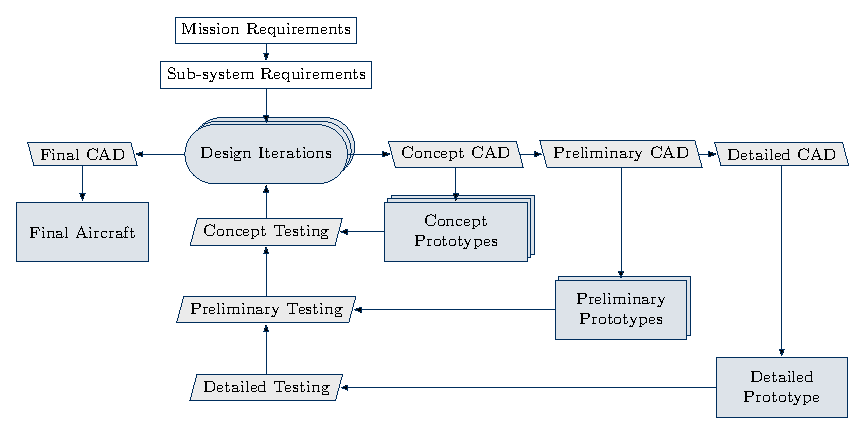
\includegraphics[width=0.6\textwidth]{manufacturing_flow}
	} %NOTE: IFF YOU COMMENT OUT THE \RAISEBOX LINE ABOVE, COMMENT OUT THIS LINE TOO.
	\caption{Our 3-phase design, build, fly plan enables a more robust final aircraft.}
	\label{fig:manufacturingplan}
\end{wrapfigure}

Our manufacturing flow follows the outline found in \cref{fig:plannedtiming} which includes three design-build-fly phases.  \Cref{fig:manufacturingplan} shows this flow with more clarity.  Note that for all phases, CAD will commence roughly a week after design starts, prototyping a week after that.

\subsubsection{Phase 1} We began with a conceptual design along with conceptual CAD, from which we have built concept prototypes to be used in testing as described below. {\color{BYUred}[ADD A DETAIL ABOUT MATERIALS AND/OR PROCESSES.]}

\subsubsection{Phase 2} We are currently beginning our preliminary design and CAD from which we will build preliminary prototypes for testing. {\color{BYUred}[ADD A DETAIL ABOUT MATERIALS AND/OR PROCESSES.]}

\subsubsection{Phase 3} Around the new year, we will start on our detailed design and CAD, which will lead to our final testing prototypes.  After polishing the design and CAD after final testing, we will manufacture our final competition aircraft. {\color{BYUred}[ADD A DETAIL ABOUT MATERIALS AND/OR PROCESSES.]}



%%%%%%%%%%%%%%%%%%%%%%%%%%%%%%%%
%%%% - Critical Processes - %%%%
%%%%%%%%%%%%%%%%%%%%%%%%%%%%%%%%
\subsection{Critical Processes}
\label{ssec:CriticalProcesses}

{\color{BYUred}[YOU NEED TO DISCUSS THE CRITICAL PROCESSES AND TECHNOLOGY BASED ON HOW YOU'VE DECIDED TO MANUFACTURE THINGS THIS YEAR.  FOAM CUTTING? 3D PRINTING? LASER CUTTING? ETC.]}
\lipsum[3]




%%%%%%%%%%%%%%%%%%%%%%%%%%%%%%%%%%%%%%%%%%%%%%%%%%%%%%%%%%%%%%%%%%%%%%%%%%%%%%%%%%%%%%%%%
%%%%%%%%%%%%%%%%%%%%%%%%%%%%%%          TESTING PLAN         %%%%%%%%%%%%%%%%%%%%%%%%%%%%
%%%%%%%%%%%%%%%%%%%%%%%%%%%%%%%%%%%%%%%%%%%%%%%%%%%%%%%%%%%%%%%%%%%%%%%%%%%%%%%%%%%%%%%%%

\section{Testing Plan} % (15 points)
\label{sec:TestingPlan}
% Section Requirements:
% 1) Component and ground test plan
% 2) Flight test plan 

As mentioned in \cref{ssec:ManufacturingFlow} and shown in \cref{fig:plannedtiming}, each of our design and build iterations culminate in testing.  Testing is divided into two categories as follows:
{\color{BYUred}[NEED TO FLESH OUT DETAILS BELOW BASED ON THE SPECIFICS OF THE COMPETITION AND YOUR CONCEPTUAL DESIGN.]}


%%%%%%%%%%%%%%%%%%%%%%%%%%%%
%%%% - Ground Testing - %%%%
%%%%%%%%%%%%%%%%%%%%%%%%%%%%
\subsection{Component/Ground Test Plan}
\label{ssec:GroundTestingPlan}

For all phases, ground testing will start roughly a week after prototyping has commenced. 

\subsubsection{Phase 1} We began by testing a quick series of concept prototypes for our {\color{BYUred}[PAYLOAD, WING FOLDING MECHANISM, LAUNCH STATION, OR WHATEVER THEY ARE THIS YEAR]} in order to quickly narrow down our brainstorming to the most viable solutions.

\subsubsection{Phase 2} In our preliminary testing phase, we will be looking at functioning prototypes of {\color{BYUred}[PAYLOAD, WING FOLDING MECHANISM, LAUNCH STATION, OR WHATEVER THEY ARE THIS YEAR]} in order to nail down the major details of the design.  This will prepare us for integration in the next phase.  In this phase, we will also be begin performing preliminary wind tunnel testing to validate our propulsion system. In addition, we will perform preliminary structural testing of our anticipated wing and other critical structures.

\subsubsection{Phase 3} Finally, we will integrate all the components and do dry runs of the ground mission, as well as final wind tunnel and structural testing to validate our detailed computational analyses.





%%%%%%%%%%%%%%%%%%%%%%%%%%%%
%%%% - Flight Testing - %%%%
%%%%%%%%%%%%%%%%%%%%%%%%%%%%
\subsection{Flight Test Plan}
\label{ssec:FlightTestingPlan}

In all phases, flight tests will typically take place at the end of the phase, in the week following the termination of the prototyping.

\subsubsection{Phase 1} Flight testing began with our concept prototype: a hand-launched, unpowered, uncontrolled glider.  Our primary goals for the concept test were to validate our static stability and general structural calculations, as well as illuminate any gotchas we may have missed in our initial design phase.

\subsubsection{Phase 2} Our preliminary flight test prototype will be a powered, controlled aircraft, though without the full competition functionality.  Our goal for the preliminary test is to validate our preliminary designs before moving on to detailed design aspects and full system integration, as well as note any unexpected behavior in the aircraft dynamic responses. 

\subsubsection{Phase 3} Our detailed design prototype will be complete enough that if desired, we could compete without building another iteration. Our goal for the final testing phase will be to fly the complete mission sequence, allowing for any final fine-tuning of the design before building our competition aircraft.







%%%%%%%%%%%%%%%%%%%%%%%%%%%%%%%%%%%%%%%%%%%%%%%%%%%%%%%%%%%%%%%%%%%%%%%%%%%%%%%%%%%%%%%%%
%%%%%%%%%%%%%%%%%%%%%%%%%%%%%%          BIBLIOGRAPHY         %%%%%%%%%%%%%%%%%%%%%%%%%%%%
%%%%%%%%%%%%%%%%%%%%%%%%%%%%%%%%%%%%%%%%%%%%%%%%%%%%%%%%%%%%%%%%%%%%%%%%%%%%%%%%%%%%%%%%%
%Bibliography (5 Points)
%\item List of all published works referenced in the text must be present in this section.
%\item Any material taken from a published source in all previous sections must have a numerical subscript corresponding to the appropriate citation in this section.
%\item References should appear in numerical order.
%\item Format should match AIAA provided guidelines:

\bibliography{ref}{}
\bibliographystyle{aiaa}

\end{document}